\chapter{QCD Bound States}
\label{chap:BSE}
\section{Bethe-Salpeter equation}
\label{bse}
Bound states in QCD are composite color-scalar objects made of color-carrying particles. Starting from common two-body state $q \bar q$ like meson and three-body state $qqq$ like baryon, and ending with exotic not-yet-detected-but-possibly-existing states like tetraquarks $qq \bar q \bar q$, glueballs $GG$ and hybrids $qqG$. Due to usual form of propagator of massive particle $\frac{1}{p^2 + M^2}$ a bound state produce a pole in the scattering amplitude in the corresponding channel. For a composite bound state, the pole can not be generated by any finite sum of Feynman diagrams \cite{9780471353867}, but only by infinite series. However it is not possible in general, so instead we may consider to strive for an infinite sum of diagrams of a particular class, which are we assume to be dominant and crucial for a given process (i.e. all ladder diagrams). This can be archived by finding an appropriate integral equation, the solutions of which can be interpreted as the result of such particular summation. \\

	In order to derive aforementioned integral equation let us consider the \DSE for quark-antiquark scattering amplitude:
\beqa
	M(p,q;P) = K(p,q;P) + \int \frac{d^4k}{(2\pi)^4} K(p,k;P) G(k,P) M(k,q;P)\;,
	\label{bse:M_DSE}
\eeqa
where $M(p,q;P)$ is the scattering amplitude, $G(k,P)$ is two-quark full propagator, $K(p,q;P)$ is the two-body irreducible scattering kernel. This equations is illustrated diagrammatically on Fig. \ref{fig:M_DSE}.
\begin{figure}[H]
\tiny
 \begin{center}
  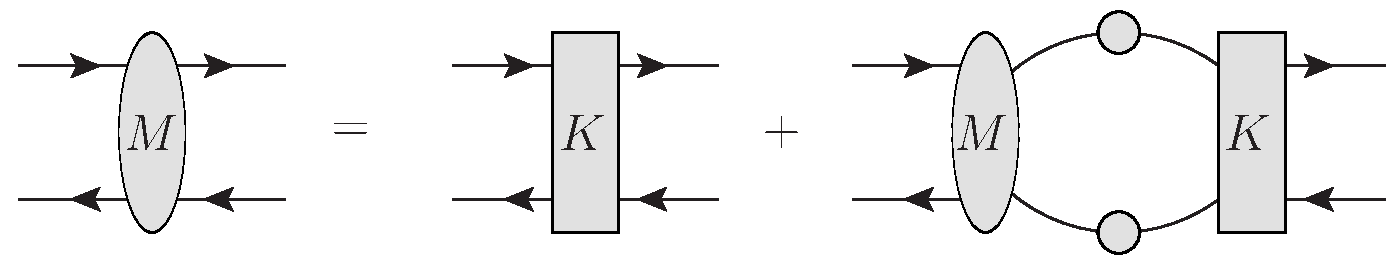
\includegraphics[width=0.95\textwidth]{figures/M_DSE}
 \end{center}
 \caption{\footnotesize \DSE  of quark-antiquark scattering amplitude. The dots on quark lines denote dressed (full) quark propagators }\label{fig:M_DSE} 
\end{figure}
If the kernel is "small", so that the perturbation series converge, the solution of Eq. (\ref{bse:M_DSE}) can be obtained by iteration. The following Born series schematically take the form:
\beqa
	M = K + \int KGK + \int \int KGKGK + \;...\; + \left(  \int KG \right)^n K +\; ...
	\label{bse:M_sum}
\eeqa

After replacing the integrals in Eq. (\ref{bse:M_sum}) by sums over discrete points in momentum, so that $K$ and $M$ are matrices and $G$ a diagonal matrix, when the Eq. (\ref{bse:M_sum}) can be formaly considered as a geometric sum, giving:
\beqa
	M &=& K + KGK + KGKGK + \;...\; + (KG)^n K +\; ... \\
	 &=& (1-KG)^{-1}K
	 \label{bse:M_sum2}
\eeqa
This expressions is similar to the simple complex function:
\beqa
	f(z)=\frac{z}{1-z}\;,
\eeqa
which is the unique analytic continuation of the series:
\beqa
	f(z)=\sum_n z^n\;,
\eeqa
from the unit circle $|z|<1$ to the region outside, $|z|\geq 1$, with the pole at $z=1$. In case $z$ being a matrix, one can generalize that $z$ has the eigenvalue $\lambda$ equal to one, so that the corresponding condition can be written as:
\beqa
	\mathbf{e} = z \mathbf{e}\;,
\eeqa
where $\mathbf{e}$ is the eigenvector. Therefore in case of Eq. (\ref{bse:M_sum2}) the condition for a pole in the scattering amplitude $M$ is following:
\beqa
	\Gamma(p;P) = \int_k K(p,k;P)G(k,P)\Gamma(k;P)\;,
\eeqa
here $\int_k$ denotes 4-momenta integration with appropriate weight. Apparently, this is the integral equation for a bound state, and $\Gamma$ refers to the bound state wave function. As a final step we need to write explicitly the two-quark full propagator $G=S\Gamma S$, so the equation writes as:
\beqa
	\Gamma^{(\mu...)}_{tu}(p;P) = \lambda(P^2) \int \frac{d^4 k}{(2\pi)^4} K_{tu;rs}(p,k;P)\left[ S(k_+)\Gamma^{(\mu...)}(k;P)S(k_-)\right]_{sr}\;,
	\label{bse:BSE_gen}
\eeqa
where the $\lambda(P^2)$ is eigenvalue. This is the \textit{homogeneous (on-shell)} Bethe-Salpeter equation (BSE) \cite{PhysRev.84.1232, PhysRev.84.350} and the function $\Gamma$ is vertex function, whose dressing functions are so-called the Bethe-Salpeter Amplitudes (BSA). The $tu;rs$ denote a relevant Dirac indexes and $(\mu...)$ reflect the Lorenz structure of the wave function. We will address an explicit representations of basis tensors later. The momenta $k_+,k_-$ obey the momenta conservation law $k_+ - k_- = P$, where $P^2=-M^2_{meson}$ is the meson mass shell. This allow us to represent $k_+,k_-$ as:
\beqa
	k_+ &=& k + \zeta P\;, \\
	k_- &=& k - (1-\zeta) P\;,
\eeqa
where $\zeta \in (0,1)$ is \textit{partitioning parameter} specifying the fraction of $P$ carried by quarks. Note that the out-coming results are independent of $\zeta$, however varying this parameter may increase the numerical complexity. Therefore for quark symmetric bound states like: $\bar n n, \bar s s, \bar c c$, etc. we employ the equal partitioning $\zeta=\frac{1}{2}$. %In case of quark asymmetric meson like: $\bar n s, \bar c s$, etc. the optimal partitioning is provided in Appendix [CITE].
 The Eq. (\ref{bse:BSE_gen}) is diagrammatically given on Fig. \ref{fig:BSE_gen}.
\begin{figure}[H]
\tiny
 \begin{center}
  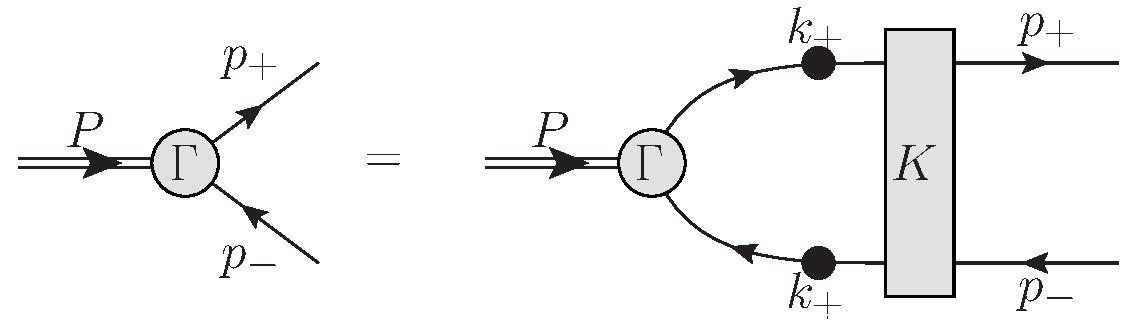
\includegraphics[width=0.95\textwidth]{figures/BSE_gen}
 \end{center}
 \caption{\footnotesize The meson \BS equations. }\label{fig:BSE_gen} 
\end{figure}
This equations is a sufficient and necessary condition for a pole to appear in $M$ 4-point Green's function at $P^2=-M^2_{meson}$. Numerically this means we need to solve inverse problem, so that we need to search for the $P^2$ such that $\lambda(P^2)=1$. \\ 

The Eq. (\ref{bse:BSE_gen}) can be transformed to \textit{inhomogeneous (off-shell)} by adding a bare term to \BSE:
\beqa
	\Gamma^{(\mu...)}(p;P) = \Gamma^{(\mu...)}_{0}(p;P) + \int_k K(p,k;P)\left[ S(k_+)\Gamma^{(\mu...)}(k;P)S(k_-)\right]\;,
	\label{bse:BSE_inhom}
\eeqa
here the $\Gamma^{(\mu...)}_{0}$ is a bare tern, which obviously must have the same Dirac and Lorenz structure as the full one $\Gamma^{(\mu...)}$, but the BSA equal one. The off-shell meson BSE is illustrated on Fig. \ref{fig:BSE_gen_offshell}.
\begin{figure}[H]
\tiny
 \begin{center}
  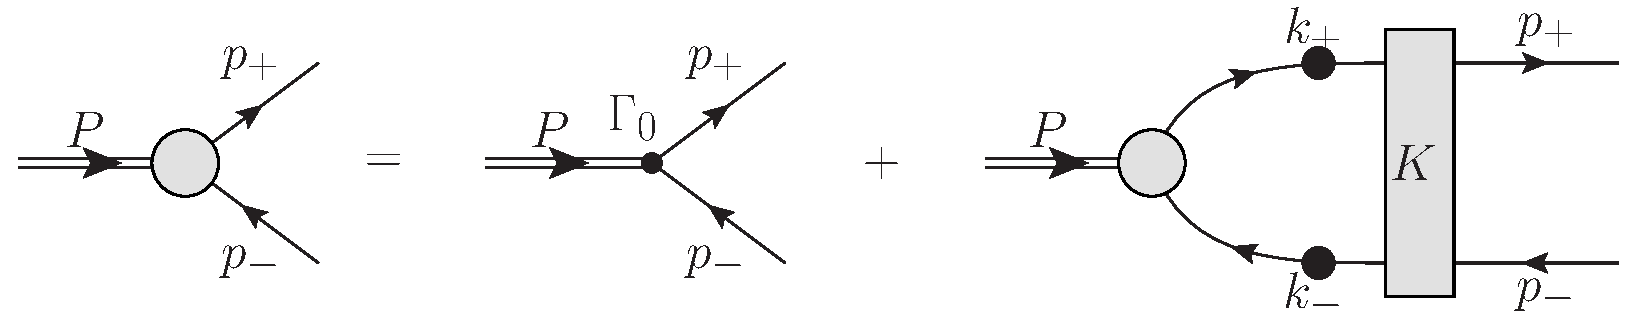
\includegraphics[width=0.95\textwidth]{figures/BSE_gen_offshell}
 \end{center}
 \caption{\footnotesize The inhomogeneous (off-shell) meson \BS equations. }\label{fig:BSE_gen_offshell} 
\end{figure}
Note that the inhomogeneous BSE given by Eq.(\ref{bse:BSE_inhom}) is no longer an eigenvalue problem, therefore has to be solved iteratively. The detailed instructions are given in Appendix \ref{app:numerics}.

\section{Total angular momentum tensor}
\label{bse:angular_tensor}
With the truncation set we are close to perform the inevitable calculations, however, the last piece from a recipe is missing. If we make a look on meson \BSE again:
\beqa
	\Gamma^{(\mu...)}_{tu}(p;P) = \lambda(P^2) \int \frac{d^4 k}{(2\pi)^4} K_{tu;rs}(p,k;P)\left[ S(k_+)\Gamma^{(\mu...)}(k;P)S(k_-)\right]_{sr}\;,
\eeqa
we see that the Dirac and Lorenz structure of $\Gamma^{(\mu...)}_{tu}(p;P)$ yet still unspecified and therefore the quantum numbers $J^{PC}$ of the meson under considerations are not yet determined. In order to do so, we choose the appropriate basis for $\Gamma^{(\mu...)}_{tu}(p;P)$, such the quantum numbers $J^{PC}$ of the meson would be clear. \\

It is well known that composite states of particles in the $\left(j,0\right)\oplus\left(0,j\right)$-representation can be constructed 
by forming direct products of the particle's representation~\cite{Joos:1962qq,Weinberg:1964cn}. For fermions, $j=1/2$, this reduces
to the Dirac spinor formalism and thus is given by the usual Dirac matrices. \\

For a meson in the rest frame with center-of-mass momentum $P_\mu$ and
relative quark momentum $p_\mu$, grouped by their transformation under parity we have
%
\begin{align}\label{eqn:scalarinvariants1}
D^{(\ONE)}&=
\left(\begin{array}{ccccc}
\;\ONE\; &
\phantom{\gamma_5}P_\mu \gamma^\mu\;&
\phantom{\gamma_5}p_\mu \gamma^\mu\;&
\phantom{\gamma_5}p_\mu P_\nu \frac{1}{2}\left[\gamma^\mu,\gamma^\nu\right]
\end{array}\right)\;, \\
%
D^{(5)}&=
\left(\begin{array}{ccccc}
\gamma_5\;&
\gamma_5 P_\mu \gamma^\mu\;&
\gamma_5 p_\mu \gamma^\mu\;&
\gamma_5 p_\mu P_\nu \frac{1}{2}\left[\gamma^\mu,\gamma^\nu\right]
\end{array}\right)\;,
\end{align}
%
for scalar, $D^{(\ONE)}$, and pseudoscalar, $D^{(5)}$, invariants respectively. Thus, for a 
bound-state of two fermions with definite parity, the basic number of scalar invariants equals
four. Furthermore, it is convenient to replace the relative momentum $p_\mu$ by
%
\begin{align}\label{eqn:transverseQ}
Q_\mu = \tau^{(P)}_{\mu\nu}\;p^\nu\;,
\end{align}
%
where $ \tau^{(P)}_{\mu\nu}=\delta_{\mu\nu}-P_\mu P_\nu/P^2$ is a transverse projector.
%
Then, appropriate scalar and pseudoscalar invariants are
%
\begin{align}\label{eqn:scalarinvariants2}
\bar{D}^{(\ONE)}&=
\left(\begin{array}{ccccc}
\;\ONE\; &
\phantom{\gamma_5}\slashed{P}\;&
\phantom{\gamma_5}\slashed{Q}\;&
\phantom{\gamma_5}\slashed{Q}\slashed{P}
\end{array}\right)\;,\;\;\;\;
%
\bar{D}^{(5)}=\gamma_5\bar{D}^{(\ONE)}\;,
\end{align}
%
which simplifies the operation of charge conjugation due to the fact that $Q\cdot P=0$.\\

Then, a bound state with zero total angular momentum and definite parity is decomposed in terms of 
four components
%
\begin{align}
\Gamma^{(Parity)}(p,t) &= \sum_{i=1}^{4} \left[A_i  \bar{D}_{i}^{(Parity)}\right]\;,
\end{align}
where $A_i$ denotes \BS amplitude - the scalar dressing function. 

For non-zero total angular momentum $J$, the $A_i$ scalar invariants
must be coupled with an angular momentum tensor. This rank $J$ tensor, $T_{a_1,\ldots a_J}$, has 
$2J+1$ independent components in three spatial dimensions, corresponding to the possible spin 
polarisations~\cite{Zemach:1968zz}. This tensor must be 
symmetric in all indices and traceless with respect to contraction of any pair of indices.
This generalizes to $3+1$ dimensions by imposing transversality of each 
index with respect to the total momentum.

Thus, to obtain a tensor corresponding to total angular momentum $J$, we construct the 
symmetric $J$-fold tensor product of a transversal projector transforming like a vector, and 
subtract traces with respect to every pair of indices. 

Then, in general a meson of spin $J>0$ and parity $P$ has eight components and is written
%
\begin{align}
\Gamma^{(Parity)}_{\mu_1\ldots\mu_J}(p,P) &= \sum_{i=1}^{4} \left[A_i Q_{\mu_1\ldots\mu_J} \bar{D}_{i}^{(Parity)}+A_{i+4} T_{\mu_1\ldots\mu_J} \bar{D}_{i}^{(Parity)}\right]\;,
\end{align}
%
where the $Q_{\mu_1\ldots\mu_J}$, $T_{\mu_1\ldots\mu_J}$ are defined below and $A_i = A_i(p,P)$. The explicit expressions for $J = 1,2,3$ can be found in Appendix \ref{app:basis}. Therefore by choosing appropriate basis can define the $J^{PC}$ quantum numbers of the meson under consideration. 

\subsection*{Axial-vector Ward Takahashi Identity}
\vspace{-0.5cm}
In previous chapter we saw how the phenomena of dynamical symmetry breaking appear in calculation, by observing a nonzero order parameter, namely, the quark condensate $\langle \bar q q \rangle$. This fact together with appearance of massless pion in the meson spectrum is a clear indication of dynamical chiral symmetry breaking in QCD, where pions are 	identified with the Goldstone bosons of the broken symmetry. The satisfaction of axial-vector Ward Takahashi Identity (axWTI) is crucial for a proper description of this phenomena within the \DS - \BSE approach \cite{Maris:1997hd}. Moreover, as we will see, the satisfaction of axial-vector Ward Takahashi Identity provides the pion vertex ansatz, shown in Eq.(\ref{dse:pion_vertex}). \\ 

The axial-vector Ward Takahashi Identity in chiral limit takes the following form:
\beqa
	-iP_\mu \Gamma^j_{5\mu}(k;P) = S^{-1}(k_+)\gamma_5\frac{\tau^j}{2} + S^{-1}(k_-)\gamma_5\frac{\tau^j}{2}\;,
	\label{bse:axWTI}
\eeqa
where the axial-vector vertex is:
\beqa
	\Gamma^j_{5\mu}(k;P) &=& \frac{\tau^j}{2}\gamma_5[\gamma_\mu F(k;P) + \gamma \cdot k k_\mu G(k;P) - \sigma_{\mu\nu}k_\nu H(k;P)] \\
	&+& f_\pi\frac{P_\mu}{P^2} \Gamma^j_\pi(k;P)\;,
	\label{bse:ax_vertex}
\eeqa
$f_\pi$ is pion weak decay constant and $\Gamma_\pi$ is general pion wave function, with the decomposition given in Eq.(\ref{dse:pion_vertex_gen}). Substituting Eq.(\ref{bse:ax_vertex}) and Eq.(\ref{dse:pion_vertex_gen}) into Eq.(\ref{bse:axWTI}) and taking limit $m^2_\pi \rightarrow 0$ one obtains the chiral limit relations between pion dressing functions and quark dressing functions \cite{Maris:1997tm}:
\beqa
	f_\pi E_\pi(k;0) = B(p^2) \\
	F(k;0) + 2f_\pi F_\pi(k;0) = A(p^2) \\
	G(k;0) + 2f_\pi G_\pi(k;0) = 2A(p^2) \\	
	H(k;0) + 2f_\pi H_\pi(k:0) = 0 \;,
	\label{bse:axWTI_relation}
\eeqa
where $E_\pi$, $F_\pi$, $G_\pi$ and $H_\pi$ are scalar dressing functions of the pion \BS amplitude. And the pion electroweak decay constant can be calculated via:
\beqa	
	f_\pi = \frac{Z_2N_C}{m^2_\pi} \int \frac{d^4 k}{(2\pi)^2} P_\mu Tr \Bigl[ \Gamma_\pi(k;P) S(k_-) \gamma_\mu \gamma_5 S(k_+) \Bigl]\;,
\eeqa
here $N_C$ is the color factor. Note however, the full pion vertex $\Gamma_\pi$ has to be properly normalized.
\section{Normalization of the BSA}
The meson bound state equation Eq.(\ref{bse:BSE_gen}) and eigenvector $\Gamma$ is defined up to arbitrary multiplicative factor, to fix which we need to impose the normalization condition on $\Gamma$. The canonical normalization \cite{1969PThPS..43....1N} has the following form:
\beqa
\notag	1 &=& 2\frac{\partial}{\partial P^2} Tr \int \frac{d^4 k}{(2\pi)^4} \Bigl[  3(\bar \Gamma(k, -Q) S(k + P/2) \Gamma(k, Q) S(k - P/2)) \;\;\;\;\;\;\;\;\;\; \\
	 &+& \int \frac{d^4 k^{\prime}}{(2\pi)^4} ( \bar \chi (k^{\prime}, -Q) K(k^{\prime} ,k;P) \chi(k,Q) ) \Bigl] \;,
	 \label{bse:Norm1}
\eeqa
where $Q^2 = - M^2_{meson}$ is fixed on mass shell and the Bethe-Salpeter wave-function is defines as:
\beqa
	\chi(k;P) = S(k + P/2)\Gamma(k;P)S(k - P/2)
\eeqa
The charge conjugated vertex function $\bar \Gamma$ is given by:
\beqa
	\bar \Gamma(k;P) = C\Gamma^{T}(-k;P)C^{-1}\;,
\eeqa
here $C=-\gamma_2\gamma_4$ is a charge conjugation matrix and index $T$ denotes the transpositioning. \\

Although the Eq.(\ref{bse:Norm1}) is a valid way to normalize $\Gamma$, it requires significant numerical efforts, since for it involves double momenta integration. Therefore it is useful to consider alternative way to normalize BSA, given by \cite{PhysRev.138.B1182,PhysRev.139.AB1,Fischer:2009jm}:
\beqa
	\Bigl( \frac{1}{\lambda}\frac{\partial \lambda}{\partial P^2} \Bigl)^{-1} = \int \frac{d^4 k}{(2\pi)^4} Tr \Bigl[ \bar \Gamma(k, -P) S(k + P/2) \Gamma(k, P) S(k - P/2)) \Bigl]\;,
	\label{bse:Norm2}
\eeqa
where the eigenvalue $\lambda=1$ at $P^2=-M^2_{meson}$. This normalization equations is beneficial, since it requires only one-loop integration and independent of the employed truncation.

\section{Scattering kernel K}
So far we discussed a general meson \BSE without specifying the truncation of BSE, which uniquely defined by truncation imposed on quark \DSE before. The reason for such connection is that the solutions of pion BSE must fulfil the axial-vector Ward Takahashi Identity in order to provide the dynamical chiral symmetry breaking and fulfil Gell-Mann-Oakes-Renner relation (GMOR), given by Eq.(\ref{qcd_low:GMOR}) in case of the explicit chiral symmetry breaking. \\
\begin{figure}[H]
\tiny
 \begin{center}
  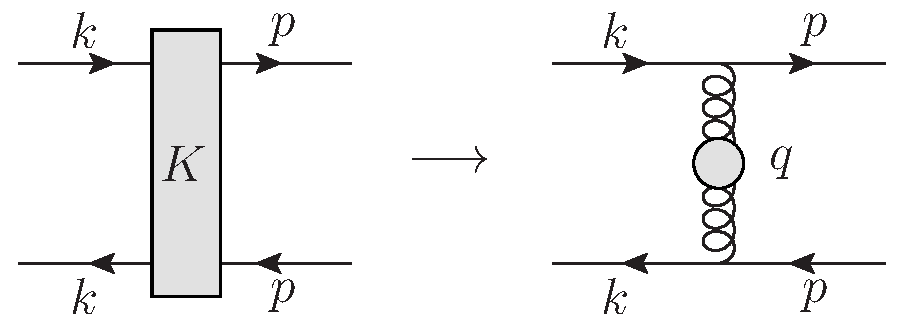
\includegraphics[width=0.75\textwidth]{figures/RL_kernel}
 \end{center}
 \caption{\footnotesize Rainbow-ladder effective one gluon exchange kernel. The filled dot represents the effective dressing via $\alpha_{\mathrm{eff}}(q^2)$. }\label{fig:RL_kernel} 
\end{figure}
In case of effective one gluon exchange also known as rainbow-ladder truncation as it was discussed in the previous chapter, the two-body scattering kernel $K(p,k;P)$ takes the following form:
\beqa
	K_{tu;rs}(p,k;P) = Z_2^2 \Bigl( \delta^{\mu\nu} - \frac{q^\mu q^\nu}{q^2} \Bigl)  \frac{\alpha_{\mathrm{eff}}(q^2)}{q^2}
	\Bigl[ \frac{\lambda^a}{2}\gamma^\mu \Bigl]_{ts} 
	\Bigl[ \frac{\lambda^a}{2}\gamma^\nu \Bigl]_{ru} \;,
	\label{bse:RL_kernel}
\eeqa
where $\lambda^a$ are Gell-Mann matrices, the $q=p-k$ is relative momentum, the indexes $\{tu;rs\}$ denote explicitly Dirac indexes, $Z_2$ is renormalization constant from quark DSE and $\alpha_{\mathrm{eff}}(q^2)$ is the same model for effective coupling as in Eq.(\ref{dse:MT_model}), used with the same parameters as for quark DSE calculation. This Eq. (\ref{bse:RL_kernel}) kernel is illustrated diagrammatically on Fig. \ref{fig:RL_kernel}. \\

In case of the unquenching pion cloud effect we need to introduce an additional contribution to the two body kernel, so can be represented as a sum:
\beqa
	K(p,k;P) = K^{gluon}(p,k;P) + K^{pion}(p,k;P)\;,
	\label{bse:PS_kernel}
\eeqa
where $K_{gluon}(p,k;P)$ is given by Eq.(\ref{bse:RL_kernel}) and $K_{pion}(p,k;P)$ is effective one pion exchange scattering kernel. The explicit view of $K_{pion}(p,k;P)$ takes the following form \cite{Fischer:2008wy,Fischer:2008sp}:
\beqa
	K^{pion}_{tu;rs}(p,k;P) &=& \frac{1}{4}[\Gamma^j_\pi]_{ru}  \left( \frac{p+k-P}{2};p-k \right)[Z_2 \tau^j \gamma_5]_{ts} D_\pi(q^2)\\
\notag	&+& \frac{1}{4}[\Gamma^j_\pi]_{ru}  \left( \frac{p+k-P}{2};k-p \right)[Z_2 \tau^j \gamma_5]_{ts} D_\pi(q^2) \\
\notag 	&+& \frac{1}{4}[\Gamma^j_\pi]_{ru}  \left( \frac{p+k+P}{2};p-k \right)[Z_2 \tau^j \gamma_5]_{ts} D_\pi(q^2) \\
\notag 	&+& \frac{1}{4}[\Gamma^j_\pi]_{ru}  \left( \frac{p+k+P}{2};k-p \right)[Z_2 \tau^j \gamma_5]_{ts} D_\pi(q^2) \;,
	\label{bse:pion_kernel}
\eeqa
here $\tau^j$ is a $SU(2)$ isospin Pauli matrices and the pion propagator $D_\pi$ in the same form as it was used in quark DSE:
\beqa
	D_\pi(q^2)=\frac{1}{q^2 + m^2_\pi}
\eeqa
The extended kernel in Eq.(\ref{bse:PS_kernel}) is represented illustratively on Fig. \ref{fig:PS_kernel}..
\begin{figure}[!]
\tiny
 \begin{center}
  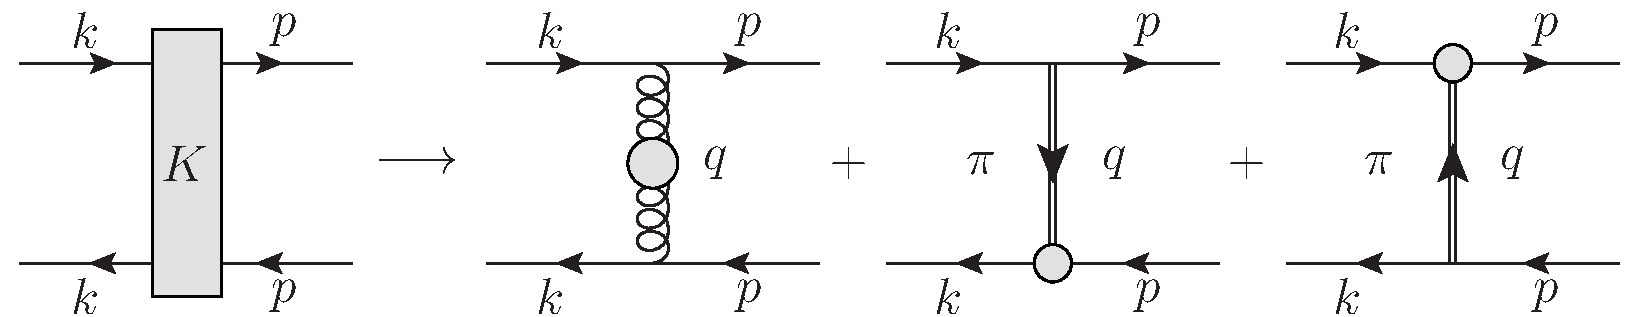
\includegraphics[width=0.99\textwidth]{figures/PS_kernel}
 \end{center}
 \caption{\footnotesize Rainbow-ladder effective one gluon and pion exchange kernel. The double line represents the pion propagator $D_\pi$ and filled dots on pion exchange diagrams denote pion vertex $\Gamma_\pi$. }
 \label{fig:PS_kernel} 
\end{figure}
However, alike in case of quark \DSE, as a pion vertex $\Gamma_\pi$ we employ the same approximation as we did in quark DSE in previous chapter:
\beqa
	\Gamma_\pi(p;P) = \gamma_5 E(p;P) = \gamma_5\frac{B(p^2)}{f_\pi}
	\label{bse:pion_vertex}
\eeqa
This approximation has negligible difference, since the first pion amplitude $E(p;P)$ is dominant, but provides the significant numerical simplification. Apparently, the Eq.(\ref{bse:pion_vertex}) naturally follows from Eq.(\ref{bse:axWTI_relation}). Recall, for the high pion mass calculations we used explicitly calculated first pion amplitude $E(p;P)$ in rainbow-ladder approach. \\

Finally, note that the interaction kernel Eq.~(\ref{bse:pion_kernel}) is not the 
full story in terms of diagrams. If the kernel were derived by the usual 
'cutting of diagrams' procedure as e.g. in a 2PI approach \cite{Munczek:1994zz}, 
a diagram would appear containing two internal pions. Such a diagram 
contains the important physics of opening up two-pion decay channels for certain
kinematics, relevant for example in the vector-meson sector. At present the resulting 
two-loop diagrams in the quark-antiquark interaction have not been addressed in the
DSE/BSE approach due to the numerical complexity involved. While a more complete approach finally has 
to deal with the two-loop diagram, in this exploratory calculation we will 
resort to the ladder contribution only.   \\

\section{Fadeev equation}
The 3-body bound state equation can be derived in a similar way as a meson BSE in Section \ref{bse}. One has to consider the \DSE for the three-quark scattering amplitude $M_(qqq)$ and applying the same idea as of dominant bound state pole contribution to $M_(qqq)$, one can derive the 3-body bound state equation, so-called Faddeev equation, that defines the mass and internal structure of baryons. Within Faddeev equation framework were performed covariant three-body calculations of nucleon, delta and omega masses \cite{Eichmann:2009qa,Eichmann:2009en,SanchisAlepuz:2011jn} as well as their electromagnetic elastic and transition form factors \cite{Eichmann:2011vu,Eichmann:2011aa,Sanchis-Alepuz:2013iia}.
  The Faddeev equation in its explicit form reads as:
\begin{equation}\label{fad:3bBSEcompact}
\Psi = -i\widetilde{K}^{(3)}~G_0^{(3)}~\Psi + \sum_{a=1}^3 -i\widetilde{K}_{(a)}^{(2)}~G_0^{(3)}~\Psi\,,
\end{equation}
where $\widetilde{K}^{(3)}$ and $\widetilde{K}^{(2)}$ are the three- and two-body interaction kernels, respectively, and $G_0$ represents the product of three fully-dressed quark propagators $S$. We used here a compact notation where indices have been omitted and we assume that discrete and continuous variables are summed or integrated over, respectively. 
The spin-momentum part of the full amplitude $\Psi$ depends on 
the total and two relative momenta of the three valence quarks inside 
the baryon. As discussed in more detail in Section \ref{subsec:internal_composition}, 
this amplitude contains all possible spin and orbital angular momentum contributions.
\begin{figure*}[h]
 \begin{center}
  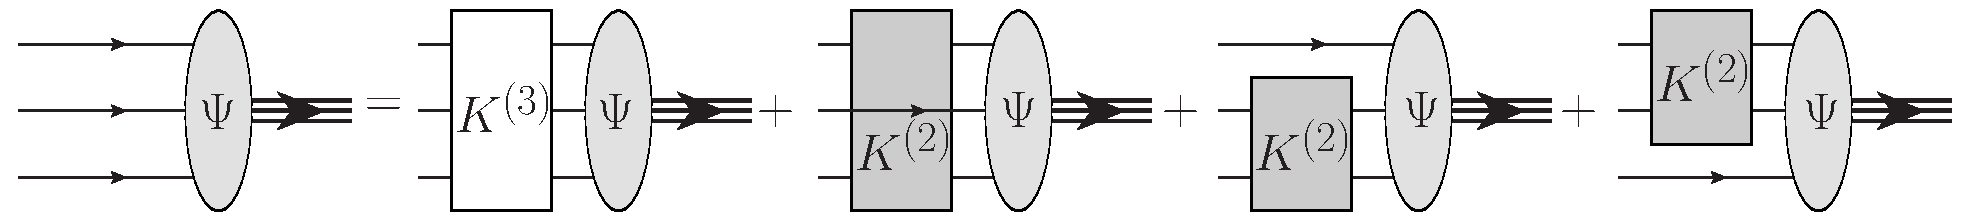
\includegraphics[width=0.99\textwidth]{figures/Faddeev}
 \end{center}
 \caption{Diagrammatic representation of the three-body Bethe-Salpeter equation.}\label{fig:faddeev_eq}
\end{figure*}
To solve the system formed by equations (\ref{fad:3bBSEcompact}) one needs to know the interaction kernels and the full quark-gluon vertex. The latter could in principle be obtained from the infinite system of coupled DSEs and BSEs of QCD. In practice, however, this system has to be truncated into something manageable, which implies that educated \textit{ans\"atze} have to be used for the Green's functions one is not solving for. 
In the quark-antiquark channel, a connection of those with the quark-gluon interaction is established
via the axial-vector Ward-Takahashi identity, which ensures the correct implementation of chiral 
symmetry in the bound state equations \cite{Munczek:1994zz,Maris:1997hd}. \\
 
When the pion exchange is included the resulting three-body equation is formally of ladder
type and explicitly given by:
\begin{flalign}\label{eq:faddeev_eq_pi}
&\hspace*{-5mm}\Psi_{\alpha\beta\gamma\mathcal{I}}(p,q,P) =~~~~~~~~~~~~~~~~~~~~~~~~~~~~~~~~~~~~~~~~~~~\nonumber\\
  \int_k & \left[
\widetilde{K}_{\beta\beta'\gamma\gamma'}(k)~S_{\beta'\beta''}(k_2)
S_{\gamma'\gamma''}(\tilde{k}_3)~
\Psi_{\alpha\beta''\gamma''\mathcal{I}}(1,P)\right.\nonumber\\
& + \left.
\widetilde{K}_{\alpha\alpha'\gamma\gamma'}(-k)~S_{\gamma'\gamma''}(k_3)
S_{\alpha'\alpha''} (\tilde{k}_1)~
\Psi_{\alpha''\beta\gamma''\mathcal{I}}(2,P)
\right. \nonumber\\
& + \left. 
\widetilde{K}_{\alpha\alpha'\beta\beta'}(k)~S_{\alpha'\alpha''}(k_1)
S_{\beta'\beta''}(\tilde{k}_2)~
\Psi_{\alpha''\beta''\gamma\mathcal{I}}(3,P)\right]\,\,,
\end{flalign}
with $\widetilde{K} = \widetilde{K}^{RL}-\widetilde{K}^{pion}$ and the generic index $\mathcal{I}$ in $\Psi$ refers to the bound state and the first
three Greek indices refer to the valence quarks \cite{Eichmann:2009qa,Eichmann:2009en,SanchisAlepuz:2011jn}. 
The Faddeev amplitudes depend on the total baryon momentum $P$ and two relative momenta $p$ and $q$
%
\begin{align}\label{eq:defpq}
        p &= (1-\zeta)\,p_3 - \zeta (p_1+p_2)\,, &  p_1 &=  -q -\dfrac{p}{2} +
\dfrac{1-\zeta}{2} P\,, \nonumber\\
        q &= \dfrac{p_2-p_1}{2}\,,         &  p_2 &=   q -\dfrac{p}{2} +
\dfrac{1-\zeta}{2} P\,, \nonumber\\
        P &= p_1+p_2+p_3\,,                &  p_3 &=   p + \zeta  P\,\,,\nonumber\\
\end{align}
%
with $p_1$, $p_2$ and $p_3$ the quark momenta and $\zeta$ a free momentum partitioning parameter, which is chosen to be $\zeta=1/3$ for numerical convenience. The quark propagators depend on 
the internal quark momenta $k_i=p_i-k$ and $\tilde{k}_i=p_i+k$, with $k$ the gluon momentum. Similarly, the internal relative momenta 
$(j,P) \equiv (p^{(j)},q^{(j)},P)$
for each of the three terms in the Faddeev equation are
%
\begin{align}\label{internal-relative-momenta}
p^{(1)} &= p+k,& p^{(2)} &= p-k,& p^{(3)} &= p,\nonumber\\
q^{(1)} &= q-k/2,& q^{(2)} &= q-k/2, & q^{(3)} &= q+k\,\,.\nonumber\\
\end{align} 
\\



	
	
	
	
	
	
	
	